%%%%%%%%%%%%%%%%%%%%%%%%%%%%%%%%%%%%%%%%%%%%%%%%%%%%%%%%%%%%%%%%%%%%%%
% LaTeX Example: Project Report
%
% Source: http://www.howtotex.com
%
% Feel free to distribute this example, but please keep the referral
% to howtotex.com
% Date: March 2011 
% 
%%%%%%%%%%%%%%%%%%%%%%%%%%%%%%%%%%%%%%%%%%%%%%%%%%%%%%%%%%%%%%%%%%%%%%
% How to use writeLaTeX: 
%
% You edit the source code here on the left, and the preview on the
% right shows you the result within a few seconds.
%
% Bookmark this page and share the URL with your co-authors. They can
% edit at the same time!
%
% You can upload figures, bibliographies, custom classes and
% styles using the files menu.
%
% If you're new to LaTeX, the wikibook is a great place to start:
% http://en.wikibooks.org/wiki/LaTeX
%
%%%%%%%%%%%%%%%%%%%%%%%%%%%%%%%%%%%%%%%%%%%%%%%%%%%%%%%%%%%%%%%%%%%%%%
% Edit the title below to update the display in My Documents
%\title{Project Report}
%
%%% Preamble
\documentclass[paper=a4, fontsize=11pt]{scrartcl}
%%%%%%%%%%%%%%%%%%%%%%%%%%%%%%%%%%%%%%%%%%%%%%%%%%%%%%%%%%%%%%%%%%%%%%%
%%% Packages
\usepackage[T1]{fontenc}
\usepackage{fourier}
\usepackage[english]{babel}															% English language/hyphenation
\usepackage[protrusion=true,expansion=true]{microtype}	
\usepackage{amsmath,amsfonts,amsthm} % Math packages
\usepackage[pdftex]{graphicx}	
\usepackage{url}
\usepackage{sectsty}
\allsectionsfont{\centering \normalfont\scshape}
\usepackage{amsmath}
\usepackage{graphicx}
\usepackage{amsthm}
\usepackage{amssymb}
\usepackage[colorlinks=true, allcolors=blue]{hyperref}
\usepackage[dvipsnames]{xcolor}
\newtheorem{theorem}{Theorem}[section]
\newtheorem{corollary}{Corollary}[theorem]
\newtheorem{lemma}[theorem]{Lemma}
\usepackage{float}
\usepackage[dvipsnames]{xcolor}
\usepackage{algorithm}
\usepackage{algpseudocode}
\usepackage[all]{xy}
\usepackage{mathtools}
\usepackage[
backend=biber,
style=alphabetic,
sorting=ynt
]{biblatex}
\usepackage{alltt}
\usepackage{fontawesome}
\usepackage{times}
\usepackage{xspace}
\usepackage{setspace}
\usepackage{enumitem}
\usepackage{amsmath}
\usepackage{amssymb}
\usepackage[dvipsnames]{xcolor}
%%%%%%%%%%%%%%%%%%%%%%%%%%%%%%%%%%%%%%%%%%%%%%%%%%%%%%%%%%%%%%%%%%%%%%%
%%% Custom headers/footers (fancyhdr package)
\usepackage{fancyhdr}
\pagestyle{fancyplain}
\fancyhead{}											% No page header
\fancyfoot[L]{}											% Empty 
\fancyfoot[C]{}											% Empty
\fancyfoot[R]{\thepage}									% Pagenumbering
\renewcommand{\headrulewidth}{0pt}			% Remove header underlines
\renewcommand{\footrulewidth}{0pt}				% Remove footer underlines
\setlength{\headheight}{13.6pt}
%%%%%%%%%%%%%%%%%%%%%%%%%%%%%%%%%%%%%%%%%%%%%%%%%%%%%%%%%%%%%%%%%%%%%%%
%%% Equation and float numbering
\numberwithin{equation}{section}		% Equationnumbering: section.eq#
\numberwithin{figure}{section}			% Figurenumbering: section.fig#
\numberwithin{table}{section}				% Tablenumbering: section.tab#
%%%%%%%%%%%%%%%%%%%%%%%%%%%%%%%%%%%%%%%%%%%%%%%%%%%%%%%%%%%%%%%%%%%%%%%
%%% New Commands
%%% Maketitle metadata
\newcommand{\horrule}[1]{\rule{\linewidth}{#1}} 	% Horizontal rule
\newcommand{\im}{\ensuremath{\operatorname{im}}}
\newcommand{\lm}{\ensuremath{\operatorname{LM}}}
\newcommand{\lt}{\ensuremath{\operatorname{LT}}}
\newcommand{\lc}{\ensuremath{\operatorname{LC}}}
\newcommand{\lev}{\ensuremath{\operatorname{lev}}}
\newcommand{\coker}{\ensuremath{\operatorname{coker}}}
\newcommand{\initTerm}{\ensuremath{\operatorname{in}}}
\newcommand{\mingens}{\ensuremath{\operatorname{mingens}}}
\newcommand{\lex}{\ensuremath{\operatorname{lex}}}
\newcommand{\lcm}{\ensuremath{\operatorname{lcm}}}
\newcommand{\grlex}{\ensuremath{\operatorname{grlex}}}
\newcommand{\grevlex}{\ensuremath{\operatorname{grevlex}}}
\newcommand{\id}{\ensuremath{\operatorname{id}}}
\newcommand{\multideg}{\ensuremath{\operatorname{multideg}}}
\newcommand{\Division}{\ensuremath{\operatorname{Division}}}
\newcommand{\Euclidean}{\ensuremath{\operatorname{Euclidean}}}
\newcommand{\GL}{\ensuremath{\operatorname{GL}}}
\newcommand{\onto}{\ensuremath{\twoheadrightarrow}}
\newcommand{\into}{\ensuremath{\hookrightarrow}}
\newcommand{\tab}[1]{\hspace{.2667\textwidth}\rlap{#1}}
\newcommand{\itab}[1]{\hspace{0em}\rlap{#1}}
\newcommand{\RNum}[1]{\uppercase\expandafter{\romannumeral #1\relax}}

%%% Renew Commands
\renewcommand{\deg}{\ensuremath{\operatorname{deg}}}
\renewcommand{\max}{\ensuremath{\operatorname{max}}}
\renewcommand{\to}{\ensuremath{\rightarrow}}
\renewcommand{\th}{\ensuremath{\operatorname{th}}}
\renewcommand{\det}{\ensuremath{\operatorname{det}}}

%%% Styles
\theoremstyle{definition}
\newtheorem{definition}{Definition}[section]

\theoremstyle{remark}
\newtheorem*{remark}{\textbf{Remark}}

\theoremstyle{example}
\newtheorem{example}{\textbf{Example}}[section]

\newcommand{\qedwhite}{\hfill \ensuremath{\Box}}

\newtheorem{prop}{Proposition}[section]
%%%%%%%%%%%%%%%%%%%%%%%%%%%%%%%%%%%%%%%%%%%%%%%%%%%%%%%%%%%%%%%%%%%%%%%
\title{
		%\vspace{-1in} 	
		\usefont{OT1}{bch}{b}{n}
		\normalfont \normalsize \textsc{Georgia Tech} \\ [25pt]
		\horrule{0.5pt} \\[0.4cm]
		\huge Comprehensive Exam Review - Algebra \\
		\horrule{2pt} \\[0.5cm]
}
\author{
		\normalfont 								\normalsize
        Ruiqi (Rickey) Huang                 \\\normalsize
        \today
}
\date{}
\addbibresource{references.bib}
%%%%%%%%%%%%%%%%%%%%%%%%%%%%%%%%%%%%%%%%%%%%%%%%%%%%%%%%%%%%%%%%%%%%%%%
%%% Set up
\begin{document}
\maketitle
\thispagestyle{empty}

\newpage

%%%%%%%%%%%%%%%%%%%%%%%%%%%%%%%%%%%%%%%%%%%%%%%%%%%%%%%%%%%%%%%%%%%%%%%
%%% Table of contents
\tableofcontents
\thispagestyle{empty}

\newpage

%%%%%%%%%%%%%%%%%%%%%%%%%%%%%%%%%%%%%%%%%%%%%%%%%%%%%%%%%%%%%%%%%%%%%%%
%%% Begin document
\section{Linear Algebra}

\subsection{Linear Algebra \RNum{1}}

\subsection{Linear Algebra \RNum{2}}

\paragraph{}

I consulted Sheldon Axler's ``Linear Algebra Done Right'' for review purposes \cite{axler_linear_2015}.

\subsubsection{Vector Spaces}

\paragraph{}

$\mathbb{F}$ is a generalization of $\mathbb{R}$ and $\mathbb{C}$, since they are both fields.

\begin{definition}[\textbf{list, length}]
    Suppose that n is a non-negative integer. A \textbf{list} of \textbf{length} $n$ is an ordered collection of $n$ elements. A list of lengths $n$ looks like this:
    \begin{equation}
        (x_1, \cdots, x_n).
    \end{equation}
    Two lists are equal if and only if they have the same length and the same elements in the same order.
\end{definition}

\paragraph{}

lists are always finite. Lists differ from sets in two ways: in lists, order matters and repetitions have meaning; in set, order, and repetitions are irrelevant.

\begin{definition}[$\mathbb{F}^n$]
    $\mathbb{F}^n$ is the set of all the length lists $n$ of elements of $\mathbb{F}$:
    \begin{equation}
        \mathbb{F}^n = \{(x_1,\cdots,x_n):x_j\in \mathbb{F} \text{ for } j = 1, \cdots, n\}.
    \end{equation}
    For $(x_1, \cdots, x_n) \in \mathbb{F}^n$ and $j \in \{1, \cdots, n\}$, we say that $x_j$ is $j^{\th}$ \textbf{coordinate} of $(x_1, \cdots, x_n)$.
\end{definition}

\paragraph{}

The additions in $\mathbb{F}^n$ are defined as element-wise additions, and the commutativity of the addition in $\mathbb{F}^n$ is the same as in $\mathbb{F}$.

\begin{definition}[$0$]
    Let $0$ denote the list of length $n$ whose coordinates are all $0$:
    \begin{equation}
        0 = (0, \cdots, 0)
    \end{equation}
\end{definition}

\paragraph{}

$0$ as a list is an additive identity for $\mathbb{F}^n$
\begin{equation}
    x + 0 = x,\; \forall x \in \mathbb{F}^n
\end{equation}

\paragraph{}

When we think of lists as arrows, we refer to them as \textbf{vectors}.

\begin{remark}
    Vectors are just aids to our understanding, not substitutes for the actual mathematics that we will develop.
\end{remark}

\begin{definition}[\textbf{scalar multiplication in $\mathbb{F}^n$}]
    The product of a number $\lambda$ and a vector in $\mathbb{F}^n$ is computed by multiplying each vector coordinate by $\lambda$:
    \begin{equation}
        \lambda(x_1, \cdots, x_n) = (\lambda x_1, \cdots, \lambda x_n);
    \end{equation}
    Here $\lambda \in \mathbb{F}$ and $(x_1,\cdots,x_n) \in \mathbb{F}^n$.
\end{definition}

In terms of the geometrical meaning of scalar multiples, it represents the transformations that shrink or stretch a vector x by a factor of $\lambda$.

If $\lambda$ is negative and $x$ is a vector in $\mathbb{R}^2$, then $\lambda x$ is the vector that points in the direction opposite to that of $x$ and whose length is $\lvert \lambda \rvert$ times the length of $x$, as shown here.

Before defining the formal definition of the vector spaces, we should first explain the definition of addition and scalar multiplication.

\begin{definition}
    Let $V$ be a set of elements in $\mathbb{F}^n$. An addition in $V$ is a function that assigns an element $u+v\in V$ to each pair of elements $u,v \in V$. A scalar multiplication in a set $V$ is a function that assigns an element $\lambda v \in V$ to each $\lambda \in \mathbb{F}$ and each $v \in V$.
\end{definition}

\begin{definition}
    A vector space is a set $V$ along with an addition on V and a scalar multiplication on V such that the following properties hold:
    \newline
    \textbf{commutativity}
    \begin{equation}
        u + v = v + u \text{ for all } u, v \in V;
    \end{equation}
    \textbf{associativity}
    \begin{equation}
        (u + v) + w = u + (v + w) \text{ and } (ab)v = a(bv) \text{ for all } u, v, w \in V \text{ and all } a, b \in \mathbb{F};
    \end{equation}
    \textbf{additive identity}
    \begin{equation}
        \text{there exists an element } 0 \in V \text{ such that } v + 0 = v, \text{ for all } v \in V;
    \end{equation}
    \textbf{additive inverse}
    \begin{equation}
        \text{for every} v \in V\text{, there exists }w \in V \text{ such that }v + w = 0;
    \end{equation}
    \textbf{multiplicative identity}
    \begin{equation}
        1v = v \text{ for all } v \in V;
    \end{equation}
    \textbf{distributive properties}
    \begin{equation}
        a(u + v) = au + av \text{ and } (a+b)v = av + bv \text{ for all } a,b \in \mathbb{F} \text{ and all } u,v \in V.
    \end{equation}
\end{definition}

\begin{definition}[$\mathbb{F}^{\infty}$]
    $\mathbb{F}^{\infty}$ is defined as the set of all sequences of elements of $\mathbb{F}$:
    \begin{equation}
        \mathbb{F}^{\infty} = \{(x_1,x_2,\cdots)\,:\,x_j\in\mathbb{F} \text{ for } j = 1,2,\cdots\}.
    \end{equation}
    The addition and scalar multiplication in $\mathbb{F}^{\infty}$ are defined as expected
\end{definition}

We introduce a general way to produce a vector space.

\begin{definition}[$\mathbb{F}^{S}$]
    If $S$ is a set,
    \begin{itemize}
        \item Then $\mathbb{F}^{S}$ denotes the set of functions from $S$ to $\mathbb{F}$.
        \item For $f,g \in \mathbb{F}^{S}$, \textbf{sum} $f+g\in \mathbb{F}^{S}$ is the function defined by
        \begin{equation}
            (f+g)(x) = f(x) + g(x)
        \end{equation}
        for all $x \in S$.
        \item For $\lambda \in \mathbb{F}$ and $f \in \mathbb{F}^{S}$, and \textbf{product} $\lambda f \in \mathbb{F}^{S}$ is the function defined by
        \begin{equation}
            (\lambda f)(x) = \lambda f(x)
        \end{equation}
        for all $x \in S$.
    \end{itemize}
\end{definition}

\begin{example}[$\mathbb{F}^{S}$ is a vector space]
    If $S$ is the non-empty set
    \begin{itemize}
        \item The additive identity of $\mathbb{F}^{S}$ is the function $0: S \to \mathbb{F}$ defined by
        \begin{equation}
            0(x) = 0
        \end{equation}
        for all $x \in S$.
        \item For $f \in \mathbb{F}$, the additive inverse of $f$ is the function $-f: S \to \mathbb{F}$ defined by
        \begin{equation}
            (-f)(x) = -f(x)
        \end{equation}
        for all $x \in S$.
    \end{itemize}
\end{example}

\begin{remark}
    $\mathbb{F}^{n}$ and $\mathbb{F}^{\infty}$ are two special cases of $\mathbb{F}^{S}$.
    \begin{equation}
        \begin{aligned}
            \mathbb{F}^{n} &= \mathbb{F}^{1,2,\cdots,n}\\
            \mathbb{F}^{\infty} &= \mathbb{F}^{1,2,\cdots}
        \end{aligned}
    \end{equation}
\end{remark}

\begin{prop}[\textbf{Unique Additive Identity}]
    A vector space has a unique additive identity.
\end{prop}

\begin{proof}
    Suppose by contradiction that $0$ and $0'$ are both additive identities for some vector space $V$. Then
    \begin{equation}
        0 = 0 + 0' = 0' + 0 = 0'.
    \end{equation}
\end{proof}

\begin{prop}[\textbf{Unique Additive Inverse}]
    Every element in a vector space has a unique additive inverse
\end{prop}

\begin{proof}
    Let V be a vector space. Let $v \in V$. Suppose by contradiction that $w$ and $w'$ are two additive inverses of $v$. Then the
    \begin{equation}
        w = w + 0 = w + (v + w') = (w + v) + w' = 0 + w' = w'.
    \end{equation}
\end{proof}

\begin{prop}[\textbf{The Number 0 times a Vector}]
    $0v = 0$ for every $v \in V$
\end{prop}

\begin{proof}
    Let $x$ be the additive inverse of $0v$. Then for all $v \in V$
    \begin{equation}
        \begin{aligned}
            &0v = (0 + 0)v = 0v + 0v\\
            \Rightarrow &0v + x = 0v + 0v + x\\
            \Rightarrow &0 = 0v + (0v + x)\\
            \Rightarrow &0 = 0v + 0\\
            \Rightarrow &0 = 0v
        \end{aligned}
    \end{equation}
\end{proof}

\begin{prop}[\textbf{A Number times Vector 0}]
    $a0 = 0$ for every $a \in \mathbb{F}$
\end{prop}

\begin{proof}
    For all $a \in \mathbb{F}$, let $x$ be the additive inverse of $a0$. We have
    \begin{equation}
        \begin{aligned}
            &a0 = a(0 + 0) = a0 + a0\\
            \Rightarrow &a0 + x = a0 + a0 + x\\
            \Rightarrow &0 = a0 + (a0 + x)\\
            \Rightarrow &0 = a0 + 0\\
            \Rightarrow &0 = a0
        \end{aligned}
    \end{equation}
\end{proof}

\begin{prop}[\textbf{The Number $-1$ times a Vector}]
    $(-1)v = -v$ for every $v \in V$
\end{prop}

\begin{proof}
    For $v \in V$, we have
    \begin{equation}
        \begin{aligned}
            v + (-1)v = 1v + (-1)v = (1+(-1))v = 0v = 0
        \end{aligned}
    \end{equation}
    Hence, $(-1)v$ is the additive inverse of $v$. i.e. $(-1)v = -v$
\end{proof}

\begin{definition}[\textbf{Subspace}]
    A subset $U$ of $V$ is called a \textbf{subspace} of $V$ if $U$ is also a vector space (using the same addition and scalar multiplication as on $V$).
\end{definition}

\begin{prop}
    A subset $U$ of $V$ is a subspace of $V$ if and only if $U$ satisfies the following three conditions:\\
    \textbf{additive identity}
    \begin{equation}
        0 \in U
    \end{equation}
    \textbf{closed under addition}
    \begin{equation}
        u,w \in U \text{ implies } u + w \in U
    \end{equation}
    \textbf{closed under scalar multiplication}
    \begin{equation}
        a \in \mathbb{F} \text{ and } u \in U \text{ implies } au \in U
    \end{equation}
\end{prop}

\begin{proof}
    If $U$ is a subspace of $V$, then $U$ satisfies the three conditions listed above by the definition of the vector space.
    
    Conversely, suppose $U$ satisfies the three conditions above, we want to show that $U$ is a vector space. First the closure conditions make sure the addition and scalar multiplication make sense on $U$. The commutativity, associativity, and distributive properties are automatically fulfilled, since $U \subseteq V$ and $V$ is a vector space. The additive identity is $0$. For an arbitrary element $u \in U$, we could show that $-u$ is the additive inverse of the $u$, since $u + (-u) = (1+(-1))u = 0u = 0$. Hence, $U$ is a vector space.
    \end{proof}

\begin{definition}[\textbf{Sum of Subsets}]
    Suppose $U_1,\cdots,U_m$ are subsets of $V$. The \textbf{sum} of $U_1,\cdots,U_m$, denoted $U_1+\cdots+U_m$, is the set of all possible sums of elements of $U_1,\cdots,U_m$. More precisely,
    \begin{equation}
        U_1+\cdots+U_m = \{u_1+\cdots+u_m:u_1\in U_1,\cdots, u_m\in U_m\}.
    \end{equation}
\end{definition}

\begin{prop}[\textbf{Sum of Subspace is the smallest containing Subspace}]
    Suppose $U_1,\cdots,U_m$ are subspaces of $V$. Then $U_1+\cdots+U_m$ is the smallest subspace of $V$ containing $U_1,\cdots,U_m$.
\end{prop}

\begin{proof}
    It is clear that $U_1+\cdots+U_m$ is a subspace of $V$, since $0 \in U_1+\cdots+U_m$, since $0 = 0 + \cdots + 0$ for each $0$ from each $U_1, \cdots, U_m$, and $U_1+\cdots+U_m$ is closed under addition and scalar multiplication because $U_i \in V$ for all $i = 1,\cdots,m$ and $V$ is closed under addition.
    
    Clearly, each $U_i$ for $i = 1,\cdots,m$ is contained in $U_1+\cdots+U_m$ by setting corresponding elemens to $0$. Next, it suffices to show that every subspace of $V$ containing $U_1,\cdots,U_m$ contains $U_1+\cdots+U_m$. Indeed, every subspace containing $U_1,\cdots,U_m$ must contain every finite sum of elements in $U_1,\cdots,U_m$.
\end{proof}

\paragraph{}

Sums of subspaces in the theory of vector spaces are analogous to unions of subsets in set theory. Given two subspaces of a vector space, the smallest subset containing them is their sum. Analogously, given two subset of a set, the smallest subset containing them is their union. similarly, we are going to introduce an analogy of disjoint union in the theory of vector spaces.

\begin{definition}[\textbf{Direct Sums}]
    Suppose $U_1,\cdots,U_m$ are subspaces of $V$.
    \begin{itemize}
        \item The sum $U_1+\cdots U_m$ is called \textbf{direct sum} if each element of $U_1+\cdots+U_m$ can be uniquely written as a sum $u_1+\cdots+u_m$, where each $u_j$ is in $U_j$.
        \item If $U_1+\cdots+U_m$ is a direct sum, then $U_1\bigoplus\cdots\bigoplus U_m$ denotes $U_1+\cdots+U_m$, with the $\bigoplus$ notation serving as an indication that this is a direct sum.
    \end{itemize}
\end{definition}

\newpage
\section{Abstract Algebra}

I consulted Dummit and Foote's ``Abstract Algebra'' \cite{foote_abstract_2003} and Aluffi's ``Algebra Chapter 0''\cite{aluffi_algebra_2009} for reviewing purpose .

\subsection{Preliminaries}

\subsubsection{Basics}

\begin{definition}[\textbf{Injection}]
    Let $f: A \to B$, $f$ is injective or is an injection if whenever $a_1 \neq a_2$, then $f(a_1)\neq f(a_2)$.
\end{definition}

\begin{definition}[\textbf{Surjection}]
    Let $f: A \to B$, $f$ is surjective or is a surjection if for all $b \in B$ there is some $a \in A$ such that $f(a) = b$, i.e., the image of $f$ is all of $B$. Notice that since a function always maps onto its range, it is necessary to specify the codomain $B$ in order for the question of surjectivity to be meaningful.
\end{definition}

\begin{definition}[\textbf{Bijection}]
    Let $f: A \to B$, $f$ is bijective or is a bijection if it is both injective and surjective. If such a bijection exist between $A$ and $B$, we say that $A$ and $B$ are in bijective correspondence.
\end{definition}

\begin{definition}[\textbf{Left Inverse}]
    Let $f: A \to B$. $f$ has a left inverse if there is a function $g: B \to A$ such that $g \circ f: A \to A$ is the identity map, i.e., $(g \circ f)(a) = a$ for all $a \in A$. 
\end{definition}

\begin{definition}[\textbf{Right Inverse}]
    Let $f: A \to B$. $f$ has a left inverse if there is a function $g: B \to A$ such that $f \circ g: A \to A$ is the identity map, i.e., $(f \circ g)(a) = a$ for all $a \in A$. 
\end{definition}

\begin{prop}
    Let $f: A \to B$.
    \begin{itemize}
        \item The map $f$ is injective if and only if $f$ has a left inverse
        \item The map $f$ is surjective if and only if $f$ has a right inverse
        \item The map $f$ is bijective if and only if there is a function $g: B \to A$ such that $f \circ g$ and $g \circ f$ are both identity maps.
        \item If $A$ and $B$ are finite sets with the same number of elements, then $f$ is bijective if and only if $f$ is surjective if and only if $f$ is injective.
    \end{itemize}
\end{prop}

\begin{proof}
    Suppose $f$ is injective, and let $C = \im f$. Then, define a function 
    \begin{equation}
        \begin{aligned}
            h: &C \to A\\
            &c \to f^{-1}(c)
        \end{aligned}
    \end{equation}
    $h$ is well-defined, since $f$ is injective, we know that for all $c \in C$, $f^{-1}(c)$ is unique. Then for all $g: B \to A$ such that $g$ is an extension of $h$ to $B$ could be the left inverse of $g$. Indeed, for all $a \in A$, $(g \circ f)(a) = g(f(a)) = f^{-1}(f(a)) = a$, since $f(a) \in C$. 
    
    Next, suppose $f$ has a left inverse $g: B \to A$. Then $(g \circ f)(a) = a$ for all $a \in A$. Suppose by contradiction that $f$ is not injective, then there is $a_1, a_2 \in A$ such that $a_1 \neq a_2$ but $f(a_1) = f(a_2)$. Then $a_1 = (g \circ f)(a_1) = g(f(a_1)) = g(f(a_2)) = (g \circ f)(a_2) = a_2$. This lead to a contradiction to $a_1 \neq a_2$. Hence, $f$ is injective.
    
    The similar proofs for the rest of the bullet points.
\end{proof}

\begin{remark}
    In the situation of the third bullet point in the previous proposition, the function $g$ is necessarily to be unique, and we shall call it to be the two-sided inverse (or simply \textbf{inverse}) of the function $f$.
\end{remark}

\begin{definition}[\textbf{Permutation}]
    A permutation of a set $A$ is simply a bijection from $A$ to $A$.
\end{definition}

\begin{definition}[\textbf{Restriction}]
    If $A \subseteq B$ and $f: B \to C$, we denote the \textbf{restriction} of $f$ to $A$ by $f\lvert A$. When the domain we are considering is understood, we shall occasionally denote $f \lvert A$ again simply as $f$ even though they are formally different functions (their domains are different).
\end{definition}

\begin{definition}[\textbf{Extension}]
    If $A \subseteq B$ and $g: a \to C$, and there exist a function $f: B \to C$ such that $f\lvert A = g$, we shall say $f$ is an extension of $g$ to $B$ (such a map need not to exist nor be unique).
\end{definition}

\begin{definition}[\textbf{Binary Relation}]
    A \textbf{binary relation} on a set $A$ is a subset $R$ of $A \times A$ and we write $a \sim b$ if $(a,b) \in R$.
\end{definition}

\begin{definition}[\textbf{Equivalence Relation}]
    A relation $\sim$ on $A$ is said to be \textbf{equivalence relation} if it is reflexive, symmetric, and transitive.
\end{definition}

\begin{definition}[\textbf{Equivalence Class}]
    If $\sim$ defines an equivalence relation on $A$, then the equivalence class of $a \in A$ is defined to be $\{x \in A \lvert x \sim a\}$. Elements of the equivalence class of $a$ are said to be equivalent to $a$. If $C$ is said to be an equivalence class, then any elements of $C$ are \textbf{representative} of $C$.
\end{definition}

\begin{definition}[\textbf{Partition}]
    A partition of $A$ is any collection $\{A_i \lvert i \in I\}$ of nonempty subsets of $A$ ($I$ some indexing set) such that
    \begin{itemize}
        \item $A = \bigcup_{i\in I}A_i$, and
        \item $A_i \cap A_j = \emptyset$, for all $i,j \in I$ with $i \neq j$, i.e., $A$ is the disjoint union of the sets in the partition.
    \end{itemize}
\end{definition}

\begin{prop}
    Let $A$ be a non-empty set.
    \begin{itemize}
        \item If $\sim$ defines an equivalence relation on $A$, then the set of equivalence classes of $\sim$ forms a partition of $A$.
        \item If $\{A_i \lvert i \in I\}$ is a partition of $A$, then there is an equivalence relation on $A$ whose equivalence classes are precisely the sets $A_i, \, i \in I$.
    \end{itemize}
\end{prop}

\begin{remark}
    The proposition above claims that the equivalence classes and the partitions define the same thing.
\end{remark}

\newpage
\subsubsection{Properties of the integers}

\begin{prop}
    Below are some basic properties of the integers $\mathbb{Z}$
    \begin{itemize}
        \item (Well Ordering of $\mathbb{Z}$) If $A$ is some nonempty subset of $\mathbb{Z}^{+}$, there is some element $m \in A$ such that $m \leq A$, for all $a \in A$ ($m$ is called a \textbf{minimal element} of $A$).
        \item If $a,b \in \mathbb{Z}$ with $a \neq 0$, we say $a$ \textbf{divides} $b$ if there is an element $c \in \mathbb{Z}$ such that $b = ac$. In this case we write $a \lvert b$; if $a$ does not divide $b$, we write $a \nmid b$.
        \item If $a,b \in \mathbb{Z}-\{0\}$, there is a unique positive integer $d$, called the \textbf{greatest common divisor} of $a$ and $b$ (or $\gcd$ of $a$ and $b$)
        \item If $a,b \in \mathbb{Z}-\{0\}$, there is a unique positive integer $d$, called the \textbf{least common multiple} of $a$ and $b$ (or $\lcm$ of $a$ and $b$)
        \item $ab = \gcd(a,b)\lcm(a,b)$
    \end{itemize}
\end{prop}

\begin{theorem}[\textbf{Division Algorithm}]
    If $a,b \in \mathbb{Z}-\{0\}$, then there exist unique $q,r \in \mathbb{Z}$ such that
    \begin{equation}
        a = qb +r \text{ and } 0 \leq r < \lvert b \rvert,
    \end{equation}
    where $q$ is the \textbf{quotient} and $r$ the \textbf{remainder}.
\end{theorem}

\begin{proof}
    \textit{Existence}: We could give an algorithm as shown in the Algorithm \ref{alg:divAlg} to prove that there always exist such $q$ and $r$
    \begin{algorithm}[H]
        \caption{Division$[a,b,q_0]$}\label{alg:divAlg}
        \begin{algorithmic}
            \State Input: two integers $a$ and $b$, with $a \geq b$ and an integer $q_0$ satisfying $bq_0 \leq a$
            \State Output: the quotient $q$ and the remainder $r$
            \newline
            \State $q := q_0$
            \State $r := a - bq$
            \While{$r \geq \lvert b \rvert$}
                \State $q = q+1$
                \State $r = r-b$
            \EndWhile
            \State return $q,\, r$
        \end{algorithmic}
    \end{algorithm}
    Because $q$ and $r$ was computed in pairs by the algorithm and $r$ is descending by each iteration of the algorithm, we know the while loop indeed terminates. Also, since the condition of the while loop state that $r \leq \lvert b \rvert$, we know that when the while loop terminates, $r < \lvert b \rvert$.
    \newline
    \textit{Uniqueness}: Suppose by contradiction that there exist $p$ and $s$ with $p \neq q$ and $s \neq r$ such that $a = pb + s$ and $0 \leq s < \lvert b \rvert$. Then $qb + r = pb + s$, which leads $r - s = (p-q)b$. This implies $\lvert r - s \rvert = \lvert (p - q)b \rvert \leq \lvert b \rvert$. However, since $0 \leq r,s < b$, $\lvert r - s \rvert \leq b$ would lead to contradiction. Hence, the $q,r$ given by the Algorithm \ref{alg:divAlg} is unique.
\end{proof}

\begin{theorem}[Euclidean Algorithm]
    The \textbf{Euclidean Algorithm} \ref{alg:eucAlg} is an important procedure which produces the $\gcd$ of two integers $a$ and $b$ by iterating \textbf{Division Algorithm}
    \begin{algorithm}[H]
        \caption{Euclidean$[a,b]$}\label{alg:eucAlg}
        \begin{algorithmic}
            \State Input: two integers $a$ and $b$ with $a \geq b$
            \State output: the greatest common divisor of $a$ and $b$, $g = \gcd(a,b)$
            \newline
            \State $(q,r0) := \Division[a,b,q_0]$ where $q_0$ is an integer satisfying $bq_0 \leq a$
            \State $r := r0$
            \While{$r \neq 0$}
                \State $r = r0$
                \State $(q,r0) = \Division[b,r,h]$ where $h$ is an integer satisfying $bh \leq a$, and $h$ should be updated for each iteration
            \EndWhile
            \State return $r0$
        \end{algorithmic}
    \end{algorithm}
\end{theorem}

\begin{proof}
    The Algorithm \ref{alg:eucAlg} terminates since $r_0$ at each time of iteration creates a decreasing sequence of positive integers. Because the sequence could not continue indefinitely, $r$ would finally be $0$ at a certain time of iteration. Hence $r_0$ exits. It is clear that the output of the algorithm divides both $a$ and $b$ by collecting common terms. Then, suppose by contradiction that there is a common divisor of $a$ and $b$, $s$ that is larger than the output of the algorithm $r$. Then, $s$ divides each $r_0$ produced by the iterations of the algorithm. In particular, $s \mid r$, which implies $s \leq r$. This leads to a contradiction to $s > r$. Hence, $r$ is $\gcd(a,b)$.
\end{proof}

\begin{theorem}
    $\gcd(a,b)$ is a $\mathbb{Z}$-linear combination of $a$ and $b$.
\end{theorem}

\begin{proof}
    Recursively writing the element $r_n$ in Algorithm \ref{alg:eucAlg} in terms of the previous remainders (namely, use equation ($n$) to solve for $r_n = r_{n-2} - q_nr_{n-1}$ in terms of the remainders $r_{n-1}$ and $r_{n-2}$, then use equation $(n-1)$ to write $r_n$ in terms of the remainders $r_{n-2}$ and $r_{n-3}$, etc., eventually writing $r_n$ in terms of $a$ and $b$) 
\end{proof}

\begin{example}
    Suppose $a = 57970$ and $b = 10353$. We could find the greatest common divisor via Algorithm \ref{alg:eucAlg}.
        \begin{align}
            57970 &= (5)10353 + 6205 \label{eqn:2.3}\\
            10353 &= (1)6205 + 4148 \label{eqn:2.4}\\
            6205 &= (1)4148 + 2057 \label{eqn:2.5}\\
            4148 &= (2)2057 + 34 \label{eqn:2.6}\\
            2057 &= (60)34 + 17 \label{eqn:2.7}\\
            34 &= (2)17
        \end{align}
    Hence, $\gcd(a,b) = 17$
    By Equation \ref{eqn:2.7}, we could write $17 = 2057 + (-60)34$. By Equation \ref{eqn:2.6}, we could write $34 = 4148 + (-2)2057$, and substituting this into the previous expression we have $17 = (-60)4148 + (121)2057$. Similarly, we get $2057 = 6205 + (-1)4148$ from Equation \ref{eqn:2.5}, and therefore, we have $17 = (121)6205 + (-181)4148$. Then, we have $17 = (-181)10353 + (302)6205$, and finally, we have $17 = (302)57970 + (-1691)10353 = 302a + (-1691)b$
\end{example}

\begin{remark}
    The $\mathbb{Z}$-combination of $a$ and $b$ for $\gcd(a,b)$ is not unique.
\end{remark}

\begin{definition}[\textbf{Prime and Composite}]
    An element $p$ of $\mathbb{Z}^{+}$ is called a \textbf{prime} if $p > 1$ and the only positive divisor of $p$ are $1$ and $p$ (initially, the word prime will refer only to positive integers). and integer $n > 1$ is said to be \textbf{composite} if it is not prime.
\end{definition}

\begin{prop}
    If $p$ is a prime number and $p\lvert ab$ for some $a,b\in\mathbb{Z}$, then either $p \lvert a$ or $p \lvert b$.
\end{prop}

\begin{proof}
    Suppose by contradiction that $p \nmid a$ and $p \nmid b$. Then, $a = np + m$ and $b = sp + t$ for some $n,m,s,t \in \mathbb{Z}$ and $m,t < p$. Hence $ab = (np+m)(sp+t) = nsp + (nt+ms)p + mt$. We know $p \nmid mt$, since otherwise some divisor of $m$ or $t$ would be a divisor of $p$ other than $1$ and $p$. This contradicts the hypothesis that $p$ is prime. Hence, $p \nmid ab$. This is a contradiction. Therefore, either $p \lvert a$ or $p \lvert b$.
\end{proof}

\begin{theorem}[\textbf{Fundamental Theorem of Arithmetic}]
    If $n \in \mathbb{Z}, \; n > 1$, then $n$ can be factored uniquely into the product of primes, i.e., there are distinct primes $p_1,p_2,\cdots,p_s$ and positive integers $\alpha_1,\alpha_2,\cdots,\alpha_s$ such that
    \begin{equation}
        n = p_1^{\alpha_1}p_2^{\alpha_2}\cdots p_s^{\alpha_s}.
    \end{equation}
    This factorization is unique by following a certain order to arrange the factors $p_1,p_2,\cdots,p_s$.
\end{theorem}

\begin{prop}
    Suppsoe the positive integers $a$ and $b$ are expressed as products of prime powers:
    \begin{equation}
        a = p_1^{\alpha_1}p_2^{\alpha_2}\cdots p_s^{\alpha_s}, \;\; b = p_1^{\beta_1}p_2^{\beta_2}\cdots p_s^{\beta_s}
    \end{equation}
    where $p_1, p_2,\cdots, p_s$ are distinct and the exponents are $\geq 0$. Then, the greatest common divisor of $a$ and $b$ is
    \begin{equation}
        \gcd(a,b) = p_1^{\min(\alpha_1,\beta_1)}p_2^{\min(\alpha_2,\beta_2)}\cdots p_s^{\min(\alpha_s,\beta_s)},
    \end{equation}
    and
    \begin{equation}
        \gcd(a,b) = p_1^{\max(\alpha_1,\beta_1)}p_2^{\max(\alpha_2,\beta_2)}\cdots p_s^{\max(\alpha_s,\beta_s)}
    \end{equation}
\end{prop}

\begin{definition}[\textbf{Euler $\phi$-function}]
    The \textbf{Euler $\phi$-function} is defined as follows: for $n \in \mathbb{Z}^{+}$ let $\phi(n)$ be the number of positive integer $a \leq n$ with $a$ relatively prime to $n$, i.e., $\gcd(a,n) = 1$.
\end{definition}

\begin{prop}
    For primes $p$, $\phi(p) = p - 1$
\end{prop}

\begin{proof}
    Since for all primes $p$ and $n \in \mathbb{Z}^{+}, n \leq p$, only when $n = p$, $\gcd(n,p) \neq 1$. Hence, $\phi(p) = p-1$.
\end{proof}

\begin{prop}
    For primes $p$, and for all $a \geq 1$ we have the formula
    \begin{equation}
        \phi(p^a) = p^a - p^{a-1} = p^{a-1}(p-1)
    \end{equation}
\end{prop}

\begin{proof}
    Since for any $p^a$ the integers $n \in \mathbb{Z}^{+}, n \leq p$ such that $\gcd(n,p) = 1$ are those $p \nmid n$. Hence, there are $p-1$ kind of remainder when dividing such $n$ by $p$. For any single remainder, there are $\tfrac{p^a}{p} = p^{a-1}$ many integers less than $p$. Hence, there are $p^{a-1}(p-1)$ many $n$. Therefore, $\phi(p^a) = p^{a-1}(p-1)$.
\end{proof}

\begin{prop}
    The function $\phi$ is multiplicative in the sense that
    \begin{equation}
        \phi(ab) = \phi(a)\phi(b) \quad \text{if } \gcd(a,b) = 1,
    \end{equation}
    note that it is important here that $a$ and $b$ be relatively prime.
\end{prop}

\begin{lemma}
    The general formula for the values of $\phi$: if $n = p_1^{\alpha_1}p_2^{\alpha_2}\cdots p_s^{\alpha_s}$, then 
    \begin{equation}
        \begin{aligned}
            \phi(n) &= \phi(p_1^{\alpha_1})\phi(p_2^{\alpha_2})\cdots \phi(p_s^{\alpha_s})\\
            &= p_1^{\alpha_1-1}(p_1-1)p_2^{\alpha_2-1}(p_2-1)\cdots p_s^{\alpha_s-1}(p_s-1)
        \end{aligned}
    \end{equation}
\end{lemma}

\newpage
\subsubsection{$\mathbb{Z}/n\mathbb{Z}$: The Integers Modulo $n$}

\begin{definition}[\textbf{$\mathbb{Z}/n\mathbb{Z}$}]
    Let $n$ be a fixed integer. Define a relation on $\mathbb{Z}$ by
    \begin{center}
        $a \sim b$ if and only if $n\lvert (b-a)$.
    \end{center}
    This relation is clearly an equivalence relation. There are precisely $n$ distinct equivalence classes mod $n$, namely
    \begin{center}
        $\Bar{0},\,\Bar{1},\,\Bar{2},\,\cdots,\,\overline{n-1}$,
    \end{center}
    determined by the possible remainders after division by $n$ and these residue classes partition the integers $\mathbb{Z}$. The set of equivalence classes under this equivalence relation will be denoted by \textbf{$\mathbb{Z}/n\mathbb{Z}$} and called the integers modulo $n$.
    
    We define the modular arithmetic as follows: for $\Bar{a},\,\Bar{b}\in\mathbb{Z}/n\mathbb{Z}$, define their sum and product by
    \begin{center}
        $\Bar{a}+\Bar{b} = \overline{a+b}\quad$ and $\quad\Bar{a}\cdot\Bar{b} = \overline{ab}$
    \end{center}
\end{definition}

\begin{theorem}
    The operations of addition and multiplication on $\mathbb{Z}/n\mathbb{Z}$ defined above are both well defined, that is, they do not depend on the choices of representatives for the classes involved. More precisely, if $a_1,a_2 \in \mathbb{Z}$ and $b_1,b_2\in \mathbb{Z}$ with $\overline{a_1} = \overline{b_1}$ and $\overline{a_2} = \overline{b_2}$, then $\overline{a_1+a_2} = \overline{b_1+b_2}$ and $\overline{a_1a_2} = \overline{b_1b_2}$, i.e., if 
    \begin{center}
        $a_1 \equiv b_1\mod n\quad$ and $\quad a_2 \equiv b_2 \mod n$
    \end{center}
    then
    \begin{center}
        $a_1+a_2 \equiv b_1+b_2 \mod n\quad$ and $\quad a_1a_2 \equiv b_1b_2 \mod n$.
    \end{center}
\end{theorem}

\begin{proof}
    See page $10$ of the book Abstract Algebra by Dummit and Foote \cite{foote_abstract_2003}.
\end{proof}

\paragraph{}

An important subset of $\mathbb{Z}/n\mathbb{Z}$ consists of the collection of residue classes which have a multiplicative inverse in $\mathbb{Z}/n\mathbb{Z}$: 
\begin{center}
    $(\mathbb{Z}/n\mathbb{Z})^{\times} = \{\overline{a} \in \mathbb{Z}/n\mathbb{Z} \,\lvert\, \text{there exits } \overline{c} \in \mathbb{Z}/n\mathbb{Z} \text{ with } \overline{a}\cdot \overline{c} = \overline{1}\}$.
\end{center}

\begin{prop}
    $(\mathbb{Z}/n\mathbb{Z})^{\times} = \{\overline{a}\in\mathbb{Z}/n\mathbb{Z} \,\lvert\,\gcd(a,n) = 1\}$.
\end{prop}

\begin{proof}
    First, it is easy to see that if any representative of $\overline{a}$ is relatively prime to $n$ then all representatives are relatively prime to $n$ so that the set on the right in the proposition is well defined.
    
    Then, suppose $\overline{a}\in \{\overline{a}\in\mathbb{Z}/n\mathbb{Z} \,\lvert\,\gcd(a,n) = 1\}$, we want to show $\overline{a} \in (\mathbb{Z}/n\mathbb{Z})^{\times}$. This is sufficient to show $\{\overline{a}\in\mathbb{Z}/n\mathbb{Z} \,\lvert\,\gcd(a,n) = 1\} \subseteq (\mathbb{Z}/n\mathbb{Z})^{\times}$. By the Euclidean algorithm, we know that if $\gcd(a,n) = 1$, then there is $s,t \in \mathbb{Z}$ such that $as + nt = 1$, which means $as = 1 - nt$. This implies $\overline{as}=\overline{a}\cdot \overline{s} = \overline{1-nt} = \overline{1}$. Therefore, $\overline{s}$ is the inverse of $\overline{a}$. Hence, $\{\overline{a}\in\mathbb{Z}/n\mathbb{Z} \,\lvert\,\gcd(a,n) = 1\} \subseteq (\mathbb{Z}/n\mathbb{Z})^{\times}$.
    
    Finally, we need to prove the converse $(\mathbb{Z}/n\mathbb{Z})^{\times} \subseteq \{\overline{a}\in\mathbb{Z}/n\mathbb{Z} \,\lvert\,\gcd(a,n) = 1\}$. Suppose $\overline{a} \in (\mathbb{Z}/n\mathbb{Z})^{\times}$. Then, there exist $\overline{c} \in \mathbb{Z}/n\mathbb{Z}$ such that $\overline{a}\cdot\overline{c} = \overline{1}$. Suppose by contradiction that $\gcd(a,n) = b \neq 1$. Then $\gcd(ac,n) \leq b$. Hence $\overline{a} \cdot \overline{c} = \overline{ac} \neq \overline{1}$. This is a contradiction. Hence, $(\mathbb{Z}/n\mathbb{Z})^{\times} \subseteq \{\overline{a}\in\mathbb{Z}/n\mathbb{Z} \,\lvert\,\gcd(a,n) = 1\}$
    
    Thus, $(\mathbb{Z}/n\mathbb{Z})^{\times} = \{\overline{a}\in\mathbb{Z}/n\mathbb{Z} \,\lvert\,\gcd(a,n) = 1\}$
\end{proof}

\newpage
\subsection{Introduction to Groups}

\subsubsection{Basic }

\begin{definition}[\textbf{Group}]
    A group is an ordered pair $(G,\star)$ where $G$ is a set and $\star$ is a binary operation on $G$ satisfying the following axioms:
    \begin{itemize}
        \item $\star$ is associative,
        \item there exist an element $e \in G$, called an \textbf{identity} of $G$, such that for all $a \in G$ we have $a \star e = e \star a = a$,
        \item for each $a \in G$ there is an element $a^{-1}$ of $G$, called an \textbf{inverse} of $a$, such that $a \star a^{-1} = a^{-1} \star a = e$.
    \end{itemize}
    The group $(G,\star)$ is called \textbf{abelian} (or commutative) if $a \star b = b \star a$ for all $a,b \in G$.
\end{definition}

\begin{remark}
    We say $G$ is \textbf{finite group} if, in addition, $G$ is a finite set.
\end{remark}

\begin{prop}
    If $G$ is a group under the operation $\star$, then, the identity of $G$ and the inverse of any element is unique. 
\end{prop}

\begin{proof}
    Suppose there are two distinct identity $f$ and $g$ of $G$. Hence, $f\star g = g$ since $f$ is the identity. Also, $f\star g = f$ due that $g$ is the identity. Therefore $f = g$. This is a contradiction. Therefore, we know that the identity of $G$ is unique. 
    
    Let $g \in G$ be an arbitrary element. Suppose by contradiction that there are two distinct elements $h$ and $f$ in $G$ such that they are both the inverses of $g$. Hence, $g \star h = e = g \star f$. Then, $h = h \star e = h \star (g \star f) = (h \star g) \star f = e \star f = f$. This leads to a contradiction. Hence, the inverse of any element is unique.
\end{proof}

\begin{prop}
    The left and right cancellation laws hold in $G$.
\end{prop}

\begin{proof}
    This can be easily proved using the left and right multiplication of the inverses.
\end{proof}

\begin{definition}[\textbf{Order}]
    For $G$ a group and $x \in G$ define the order of $x$ to be the smallest positive integer $n$ such that $x^n = 1$, and denote that this integer by $\lvert x \rvert$. In this case $x$ is said to be of order $n$. If no positive power of $x$ is the identity, the order of $x$ is defined to be infinity and $x$ is said to be of infinite order.
\end{definition}

\begin{example}
    In the multiplicative group $\mathbb{R} - \{0\}$ or $\mathbb{Q} - \{0\}$ the element $-1$ has order $2$ and all other nonidentity elements have infinite order.
\end{example}

\begin{definition}
    Let $G = \{g_1, g_2, \cdots, g_n\}$ be a finite group with $g_1 = 1$. The multiplication table or group table of $G$ is the $n \times n$ matrix whose $i,j$ entry is the group element $g_ig_j$.
\end{definition}

\paragraph{Dihedral Group}

An important family of examples of groups is the class of groups whose elements are symmetries of geometric objects. The simplest subclass is when the geometric objects are regular planar figures.

\begin{definition}[\textbf{$D_{2n}$}]
    For each $n \in \mathbb{Z}^{+}, \, n \geq 3$ let $D_2n$ be the set of symmetries of a regular $n$-gon, where a symmetry includes the rotations and reflections that remain the $n$-gon unchanged. One can also understand the elements in $D_{2n}$ by the permutation of vertices if we label them. Now make $D_2n$ into a group by defining $st$ for $s,t \in D_{2n}$ to be the symmetry obtained by first applying $t$ then $s$ to the $n$-gon like the function compositions. The identity of $D_{2n}$ is the identity symmetry (which leaves all vertices fixed), denoted by $1$, and the inverse of $s \in D_{2n}$ is the symmetry which reverses all rigid motions of $s$. The order of $D_{2n}$ $\lvert D_{2n} \rvert = 2n$.
\end{definition}

\paragraph{Notation Conventions}

Fix a regular $n$-gon centered at the origin in an $x,\,y$ plane and label the vertices consecutively from $1$ to $n$ in a clockwise manner. Let $r$ be the rotation clockwise about the origin through $\tfrac{2\pi}{n}$ radian. Let $s$ be the reflection about the line of symmetry through vertex $1$ and origin. Then $r,\, s$ satisfy the following properties:

\begin{itemize}
    \item $1, r,r^2, \cdots r^{n-1}$ are all distinct and $r^n = 1$, so $\lvert r \rvert = n$.
    \item $\lvert s \rvert = 2$.
    \item $s \neq r^i$ for any $i$.
    \item $sr^i \neq sr^j$, for all $0 \leq i,j \leq n-1$ with $i\neq j$, so 
    \begin{equation}
        D_{2n} = \{1,r,r^2,\cdots ,r^{n-1},s,sr,sr^2,\cdots,sr^{n-1}\}
    \end{equation}
    \item $rs = sr^{-1}$. this shows $D_2n$ is non-abelian.
    \item $r^is = sr^{-i}$, for all $0 \leq i \leq n$. This indicates how to commute $s$ with powers of $r$.
\end{itemize}

Proof of the last bullet point above.

\begin{proof}
    we will show this by induction. 
    
    \textbf{Base Case:} $rs = sr^{-1}$ is clear.
    
    \textbf{Inductive Hypothesis:} Suppose $r^{k}s = sr^{-k}$,
    
    \textbf{Inductive Step:} we need to show $r^{k+1}s = sr^{-k-1}$.
    
    \begin{equation}
        \begin{aligned}
            & r^ks = sr^{-k}\\
            \Rightarrow & r(r^ks) = r(sr^{-k})\\
            \Rightarrow & (rr^k)s = (rs)r^{-k}\\
            \Rightarrow & r^{k+1}s = (sr^{-1})r^{-k} \text{ by the base case.}\\
            \Rightarrow & r^{k+1}s = sr^{-k-1}
        \end{aligned}
    \end{equation}
    Hence, For all $0 \leq i \leq n-1$, $r^is = sr^{-i}$.
\end{proof}

\begin{remark}
    One could notice that $r^n = 1$, $s^2 = 1$, and $r^is = sr^{-i}$ are three essential relations that defines the elements in $D_{2n}$. these relations are useful for the presentation notation of $D_{2n}$.
\end{remark}

\paragraph{Generators and Relations}

\begin{definition}[\textbf{Generator}]
    A subset $S$ of a group $G$ with the property that every element of $G$ can be written as a (finite) product of elements of $S$ and their inverses is called a set of \textbf{generators} of $G$. We shall indicate this notationally by writing $G = \langle S \rangle$ and say $G$ is generated by $S$ or $S$ generates $G$.
\end{definition}

\paragraph{}

Since $s \neq r^i$ for any $i$, then $D_{2n} = \langle r, s \rangle$

\begin{definition}[Presentation of a Group]
    In general, if some group $G$ is generated by a subset $S$ and there is some collection of relations, say $R_1,R_2, \cdots, R_m$ (here each $R_i$ is an equation in the element from $S \bigcup \{i\}$) such that any relation among the elements of $S$ can be deduced from these, we shall call these generators and relations a \textbf{presentations} of $G$ and write
    \begin{equation}
        G = \langle S \,\lvert\, r_1,R_2,\cdots,R_m \rangle.
    \end{equation}
    One presentation for the dihedral group $D_2n$ is then
    \begin{equation}
        D_{2n} = \langle r,s \,\lvert\, r^n = s^2 = 1, rs = sr^{-1} \rangle.
    \end{equation}
\end{definition}

\paragraph{Symmetric Groups}

\begin{definition}[\textbf{Symmetric Group $S_n$}]
    Let $\Sigma$ be any nonempty set and let $S_{\Sigma}$ be the set of all bijection from $\Sigma$ to itself. The set $S_{\Sigma}$ is a group under function composition: $\circ$.
\end{definition}

\paragraph{}

The symmetric group $S_n$ is a group of order $n!$. A \textbf{cycle} is a string of integers which representats the element of $S_n$ which cyclically permutes these integers. $S_n$ is a non-abelian group for all $n \geq 3$, but the disjoint cycles in the cycle decomposition of the permutations commute.

\paragraph{Matrix Groups}

\begin{definition}[\textbf{Matrix Groups}]
    For each $n \in \mathbb{Z}^{+}$ let $\GL_n(F)$ be the set of all $n\times n$ matrices whose entries come from $F$ and whose determinant is nonzero, i.e.,
    \begin{equation}
        {\GL}_n(F) = \{A \,\lvert\,A \text{ is an } n \times n \text{ matrix with entries from } F \text{ and } \det(A) \neq 0\}
    \end{equation}
    This is called the \textbf{general linear group of degree $n$.}
\end{definition}

\paragraph{}

The following results will be proved later but recorded now for convenience:

\begin{prop}
    (1) if $F$ is a field and $\lvert F \rvert < \infty$, then $\lvert F \rvert = p^m$ for some prime $p$ and integer $m$.
    
    (2) if $\lvert F \rvert = q < \infty$, then $\lvert \GL_n(F)\rvert = (q^n - 1)(q^ - q)(q^n-q^2)\cdots(q^n-q^{n-1})$.
\end{prop}

\paragraph{The Quaternion Group}

\begin{definition}
    The \textbf{quaternion} group, $Q_8$, is defined by
    \begin{equation}
        Q_8 = \{1,-1,i,-i,j,-j,k,-k\}
    \end{equation}
    with product $\cdot$ ccomputed as follows:
    \begin{equation}
        \begin{aligned}
            1 \cdot a &= a \cdot 1 = a, \text{ for all } a \in Q_8\\
            (-1)\cdot (-1) = 1,\,& (-1)\cdot a = a \cdot (-1) = -a, \text{ for all } a \in Q_8\\
            & i \cdot i = j \cdot j = k \cdot k =-1\\
            & i \cdot j = k, \quad j \cdot i = -k\\
            & j \cdot k = i, \quad k \cdot j = -i\\
            & k \cdot i = j, \quad i \cdot k = -j.
        \end{aligned}  
    \end{equation}
\end{definition}

\paragraph{}

$Q_8$ is a non-abelian group of order $8$.

\paragraph{Homomorphisms and Isomorphisms}

\begin{definition}[\textbf{Homomorphism}]
    Let $(G,\star)$ and $(H,\diamond)$ be groups. A map $\varphi: G \to H$ such that
    \begin{equation}
        \varphi(x \star y) = \varphi(x) \diamond \varphi(y), \text{ for all } x,y \in G
    \end{equation}
    is called a \textbf{homomorphism}.
\end{definition}

\begin{definition}[\textbf{Isomorphism}]
    The map $\varphi: G \to H$ is called an \textbf{isomorphism} and $G$ and $H$ are said to be isomorphic or of the same isomorphism type, written $G \cong H$, if
    \begin{itemize}
        \item $\varphi$ is a homomorphism (i.e., $\varphi(xy) = \varphi(x)\varphi(y)$), and
        \item $\varphi$ is a bijection.
    \end{itemize}
\end{definition}

\begin{remark}
    Intuitively $G$ and $H$ are the same group except that the elements and the operations may be written differently in $G$ and $H$.
    
    One of the central problem in mathematics is to determine what properties of a structure specify its isomorphic type. It is to prove that if $G$ is an object with some structure and $G$ has property $\mathcal{P}$, then any other similarly structured object $X$ with property $\mathcal{P}$ is isomorphic to $G$. Theorems of this type are referred to as \textbf{classification theorems}.
    
    For example, we shall prove that
    
    \begin{center}
        any non-abelian group of order $6$ is isomorphic to $S_3$.
    \end{center}
\end{remark}

\begin{prop}
        If $\varphi: G \to H$ is an isomorphism, then, in particular,
    \begin{itemize}
        \item $\lvert G \rvert = \lvert H \rvert$
        \item $G$ is abelian if and only if $H$ is abelian
        \item for all $x \in G$, $\lvert x \rvert = \lvert \varphi(x) \rvert$.
    \end{itemize}
\end{prop}

\begin{remark}
    Intuitively, we can map the generators of $G$ to any elements of $H$ and obtain a homomorphism provided that the relations in $G$ are still satisfied. This create isomorphisms using the group presentations. In particular, in vector spaces, if there is a linear transformation from a vector space $V$ to another vector space $W$ (here there are no relations to satisfy), and $V,W$ both have dimension $n$, and the vectors mapped to from the generators of $V$ span $W$ (the same generators), then this linear transformation is invertible (a vector space isomorphism).
\end{remark}.

\begin{figure}[H]
        \centering
        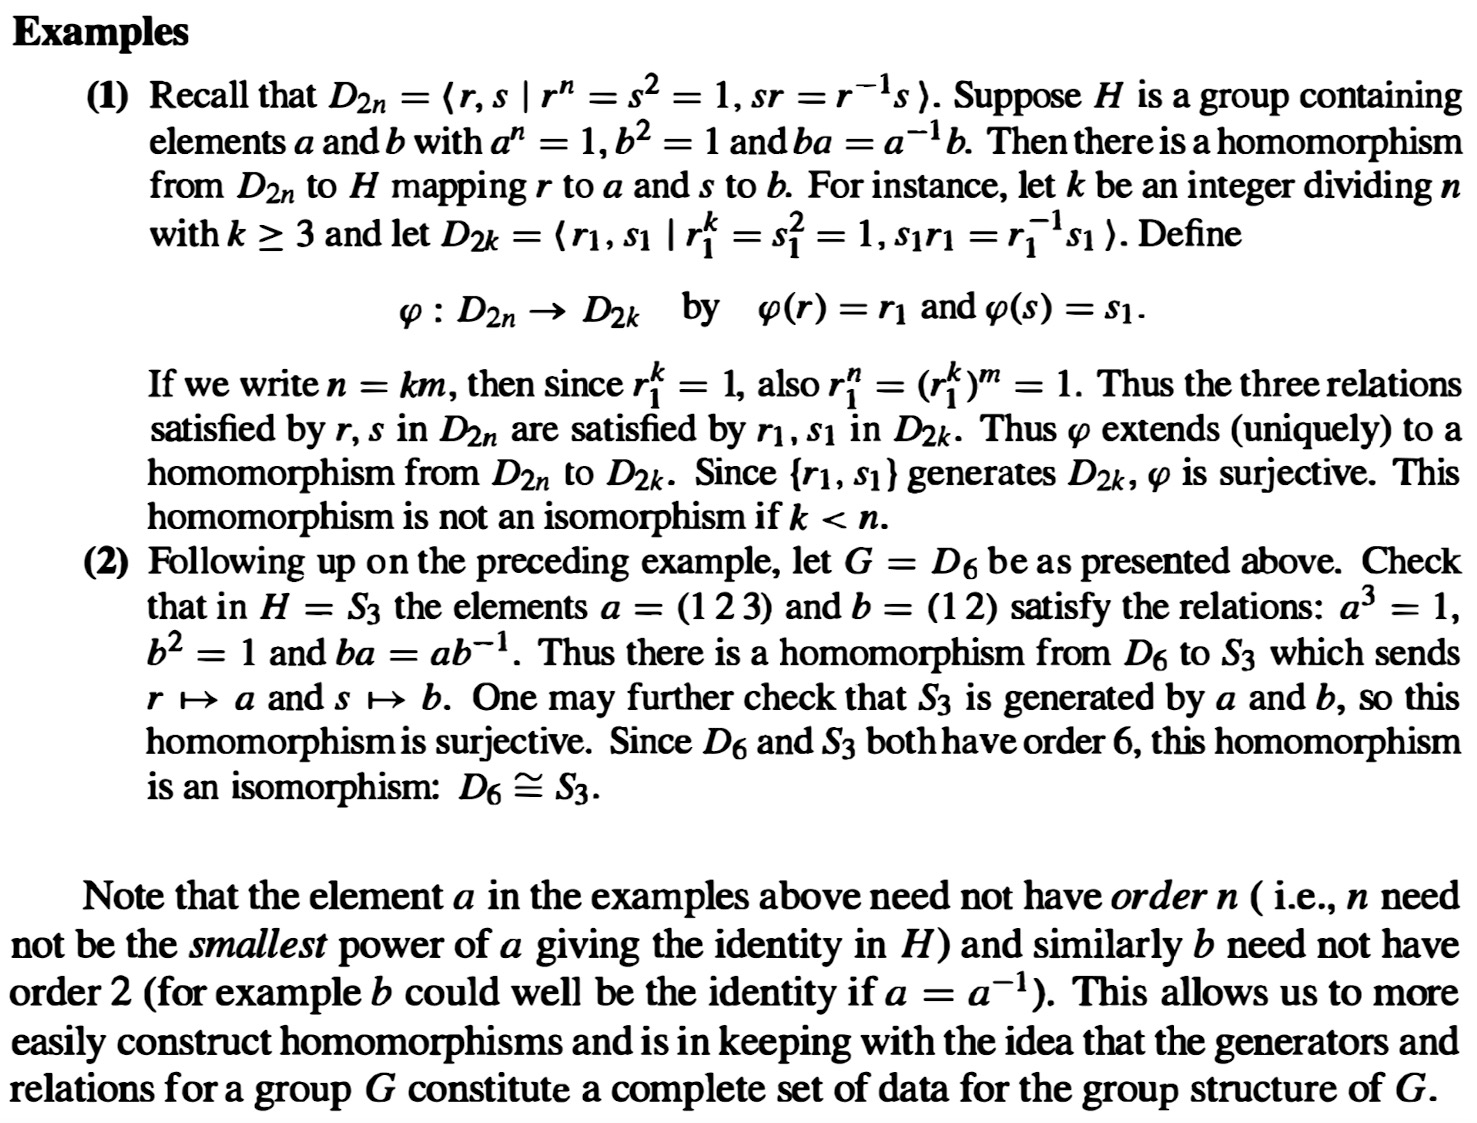
\includegraphics[width=0.9\textwidth]{1.jpeg}
        \caption{\label{fig:fig1}A Good Example}
\end{figure}

%%% End document

\newpage
\printbibliography

\end{document} 